\section{Multilagen-PVD}
\label{multilayer}

Zur Herstellung von mehrlagigen Schichten wie röntgenoptischen oder magnetischen Systemen (Riesenmagnetowiderstand GMR, Tunnelmagnetowiderstand TMR) werden Elektrodepositionen\cite{yang_pulsed_1995} und Sputter-Prozesse\cite{barshilia_characterization_2002,cammarata_nanoindentation_1990} genutzt, die beide zur Klasse der PVD-Methoden gehören.
Mit Parsivald werden deshalb Abscheidungssimulation von Kupfer-Nickel-Multilagen durchgeführt, bevor die Ergebnisse mit den Ergebnissen von rein molekulardynamischen Rechnungen verglichen werden.

Die Wahl fiel auf das Kupfer-Nickel-System aufgrund der gleichen fcc-Struktur und der ähnlichen Gitterkonstanten von \SI{3.615}{\angstrom} für Kupfer und \SI{3.5238}{\angstrom} für Nickel\cite{haynes_crc_2011}, wodurch Gitterdefekte vermieden werden und epitaktisches Wachstum möglich ist\cite{zhou_atomistic_1998}.
In MD-Simulationen von \textsc{Zhou et al.}\cite{zhou_atomistic_1998} wurden bereits Gitterdefekte und -versetzungen für Lagen von je \SI{20}{\angstrom} Dicke untersucht, doch wurden während dieser Simulationen keine amorphen Schichten beobachtet.
In dieser und weiteren Untersuchungen\cite{zhou_atomic_2001} wurden erfolgreich EAM-Potentiale benutzt, um dünne Multilagen-Systeme zu simulieren.
Dabei bildeten sich in der Simulation klar abgetrennte Lagen aus, die nur bei hoher Energie des auftreffenden Teilchens zu einer Durchmischung des Systemes führen\cite{zhou_atomistic_1998}.

\todoline{irreführend geschrieben. Letztlich kommen diese Dicken ja von den jeweiligen technologischen Erfordernissen und den Abscheideeinstellungen - das ist ja keine Größe die den Strukturen fundamental eigen ist}

In experimentellen Untersuchungen von \ce{Cu-Ni}-Multilagen wurden für Sputter-Prozesse Dop\-pel\-lagen-Dicken von \SIrange{1.6}{12}{\nano\meter}\cite{cammarata_nanoindentation_1990} und \SI{160}{\nano\meter} für Elektrodepositions-Prozesse\cite{yang_pulsed_1995} verwendet.
Eine Untersuchung der Oberfläche für gesputterte Schichten mit einer Dicke von \SI{1.5}{\micro\meter} bei Doppellagen-Dicken von \SIrange{51}{117}{\angstrom} ergab Unebenheiten an der Oberfläche mit einer Tiefe von \SIrange{30}{40}{\nano\meter}\cite{barshilia_characterization_2002}.
Damit sind die experimentellen Lagen häufig dicker als die mit Parsivald simulierten Doppel\-lagen-Dicken von \SI{2}{\nano\meter}, allerdings beschränken sich die Untersuchungen auf mechanische, magnetische oder elektronische Eigenschaften, sodass ohnehin kein direkter Vergleich mit strukturellen Daten möglich ist.
Da dickere Lagen zudem mit einer Rechenzeit von mehreren Wochen einher gehen, waren sie aufgrund der Notwendigkeit mehrerer Anpassungszyklen der Abscheidungssimulation im zeitlichen Rahmen dieser Arbeit nicht durchführbar.
Stattdessen werden die Ergebnisse mit denen anderer MD-Rechnungen verglichen.
Sofern die MD-Rechnungen mit dem benutzten EAM-Parametersatz das Zielsystem hinreichend beschreiben und eine Übereinstimmung mit der Parsivald-Simulation vorliegt, sollten auch größere Systeme effizient simuliert werden können.

\subsection{Multilagen-Simulationen mit Parsivald}

Für die Parsivald-Simulation wurde auf einen neuen EAM-Parametersatz für Kupfer-Nickel-Legierungen zurück gegriffen\cite{onat_optimized_2014}, der dem LAMMPS-Paket erst seit Kurzem beigelegt ist und deshalb noch nicht bei den Untersuchungen von Kupfer-Parametrisierungen in Abschnitt~\ref{copperpvd} betrachtet wurde.
Die weiteren Simulationsparameter wurden direkt von der Kupfer-PVD-Simu\-la\-tion übernommen, wobei die Relaxationszeiten für die MD-Rechnungen variiert wurden, um ihren Einfluss auf die Durchmischung der Schichten zu untersuchen.
Die Auftreffenergien der Atome wurden mit \SI{4.2}{\electronvolt} im unteren Bereich der Werte aus Referenz~\cite{zhou_atomistic_1998} gewählt, um das Herausschlagen von Oberflächenatomen zu vermeiden.
Die PVD-Raten wurden so gewählt, dass einzelne Lagen mit einer Dicke von \SI{1}{\nano\meter} erzeugt werden.
Abscheidungen von Lagen mit einer Dicke von \SI{5}{\nano\meter} wurden ebenfalls mit Parsivald simuliert, doch mangels verfügbarer Rechenzeit nicht eingehender untersucht.
Anhang~\ref{appendix_multilayer} enthält neben diesen Systemen auch Darstellungen von strukturellen Fehlern, die bei der Fehleinstellung der Simulationsparameter von der Simulation verursacht werden können.

Eine Untersuchung der Ergebnisse der Parsivald-Simulationen zeigt nach korrekter Parametereinstellung klar abgegrenzte epitaktische Atomlagen (Abbildungen~\ref{fig:multilayerresults}), die eine geringe Rauheit von \SI{1.2}{\angstrom} zeigen (Abbildung~\ref{fig:multilayerplots-a}), welche unterhalb der Bindungslängen liegt.
Diese Beobachtungen decken sich mit den Ergebnissen anderer Simulationen\cite{zhou_atomic_2001,zhou_atomistic_1998}.
Bei Untersuchungen der Alpha-Form konnten weder Poren noch Hohlräume gefunden werden.
Die Lagen zeigen jedoch bei geringeren Relaxationszeiten eine stärkere Durchmischung, wie in Abbildung~\ref{fig:multilayerplots-b} anhand der nach Schichthöhe aufgelösten Atomkonzentration ersichtlich ist.
In der Simulation wird die Durchmischung durch eine Unterrelaxation verursacht, bei der sich das auftreffende Atom nicht weit genug auf der Oberfläche bewegen kann, um einen günstigen Ablagerungsort zu erreichen.
Stattdessen verbleibt es in direkter Nähe zum möglicherweise ungünstigen Auftreffort, wodurch sich Unebenheiten verstärken können und somit die Durchmischung erhöht.
Ähnliche Effekte wurden von \textsc{Zhou et al.}\cite{zhou_atomistic_1998} bereits für niedrige Auftreffenergien beobachtet.
Für Systeme, die zu einer stärkeren Durchmischung neigen, sollten längere Relaxationszeiten diese zusätzlich befördern.

\begin{figure}[bp]
  \captionsetup[subfigure]{singlelinecheck=false}
  \def\subfigwidth{7cm}
  \begin{subfigure}[t]{\subfigwidth}
    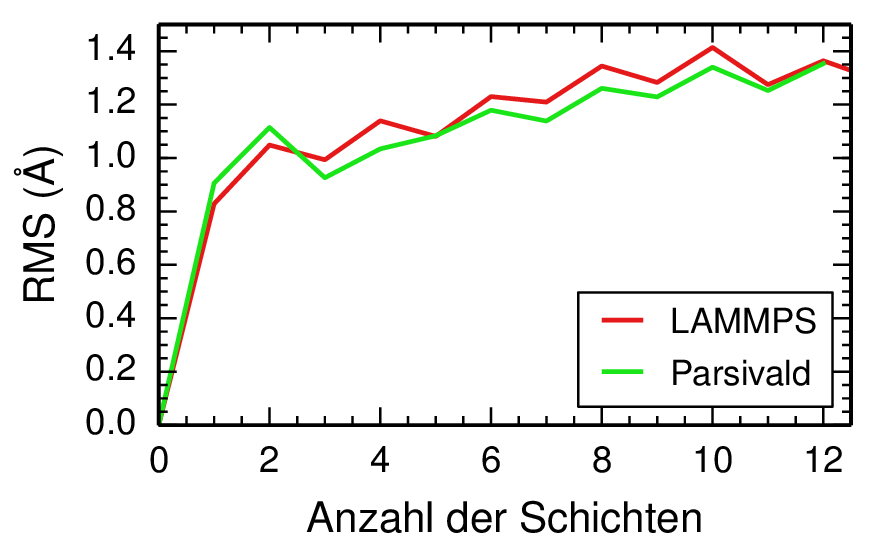
\includegraphics[width=\textwidth]{CuNi_layerroughness_comparison}
    \subcaption{
      Vergleich der Lagen-Rauheit (Abb.~\ref{fig:multilayerresults})
    }
    \label{fig:multilayerplots-a}
  \end{subfigure}
  \hfill
  \begin{subfigure}[t]{\subfigwidth}
    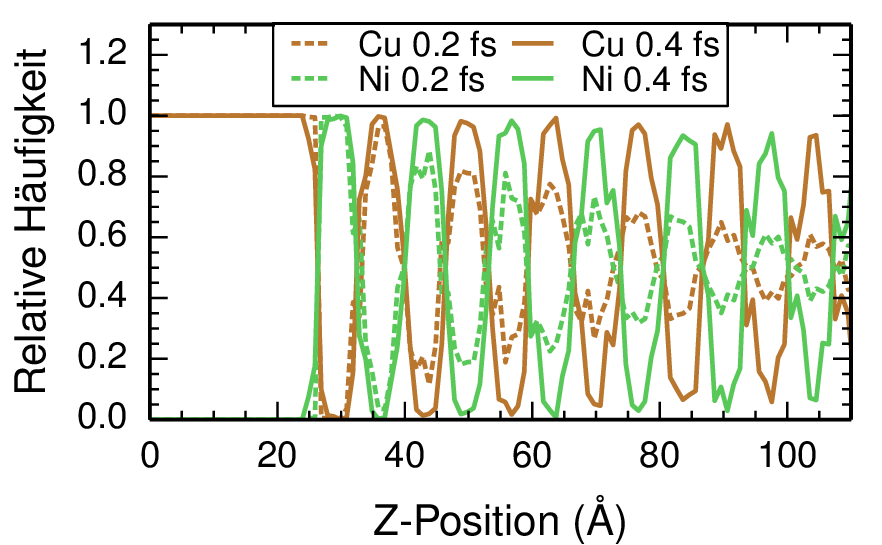
\includegraphics[width=\textwidth]{CuNi_atomdistribution_relax}
    \subcaption{Einfluss von $t_\text{relax}$ auf die Lagen-Qualität}
    \label{fig:multilayerplots-b}
  \end{subfigure}
  \caption[Rauheit und Qualität von Kupfer-Nickel-Multilagen]{
    Rauheit und Qualität von Kupfer-Nickel-Multilagen
  }
  \label{fig:multilayerplots}
\end{figure}

\subsection{Vergleich mit Ergebnissen reiner MD-Simulationen}

Zur Erzeugung von Vergleichsstrukturen wurden reine MD-Simulationen mit LAMMPS durchgeführt, welches auch von Parsivald für MD-Rechnungen als Laufzeit-Bibliothek eingebunden wird.
Dabei wurde die Größe des Substrates beibehalten und während der Simulation Atome vom oberen Rand des Simulationsraumes auf die Oberfläche aufgebracht, wofür die PVD-Raten zugunsten der Rechenzeit um mehrere Größenordnungen höher als bei Parsivald-Rechnungen gewählt werden mussten.
Dadurch sind gegenseitige Einflüsse zwischen benachbarten Abscheidungsorten nicht ausgeschlossen und können die Filmqualität durch Bildung von Nanopartikeln potentiell verringern.
Im Gegensatz zu Parsivald wird bei den reinen LAMMPS-Rechnungen der komplette Simulationsraum simultan berechnet, wodurch auch langreichweitige Effekte berücksichtigt werden.

Beim Vergleich der Ergebnisse von Parsivald und LAMMPS zeigt sich jedoch eine gute Übereinstimmung der Schichten (Abbildung~\ref{fig:multilayerresults}), die auch in den Rauheiten erkennbar ist (Abbildung~\ref{fig:multilayerplots-a}).
Sowohl die Ergebnisse der Abscheidungssimulationen mit Parsivald als auch die der LAMMPS-Rechnungen weisen Rauheiten unterhalb der Bindungslängen auf und zeigen weder Hohlräume noch Gitterdefekte.
Bei den LAMMPS-Simulationen wurde versehentlich eine leicht geringere Zahl von Atomen pro Lage adsorbiert, woraus sich ca. \SI{6}{\percent} dünnere Schichten ergeben.

\begin{figure}[tp]
  \captionsetup[subfigure]{singlelinecheck=false}

  \hspace{1.5em}
  \begin{subfigure}[c]{0.7cm}
    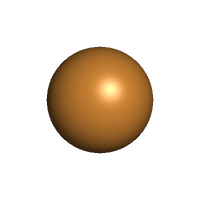
\includegraphics[width=\textwidth]{Cu}
  \end{subfigure}
  \begin{subfigure}[c]{0.7cm}
    \ce{Cu}
  \end{subfigure}
  \begin{subfigure}[c]{0.7cm}
    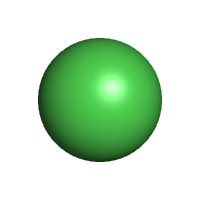
\includegraphics[width=\textwidth]{Ni}
  \end{subfigure}
  \begin{subfigure}[c]{0.7cm}
    \ce{Ni}
  \end{subfigure}

  \def\subfigwidth{7cm}
  \begin{subfigure}[t]{\subfigwidth}
    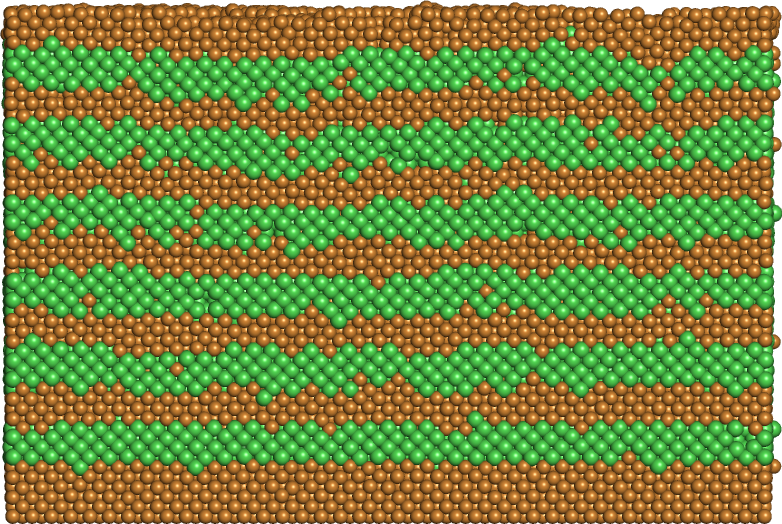
\includegraphics[width=\textwidth]{CuNi_LAMMPS_45}
    \subcaption{Profil von \ce{Cu-Ni}-Multilagen, reine MD-Simulation mit LAMMPS}
  \end{subfigure}
  \hfill
  \begin{subfigure}[t]{\subfigwidth}
    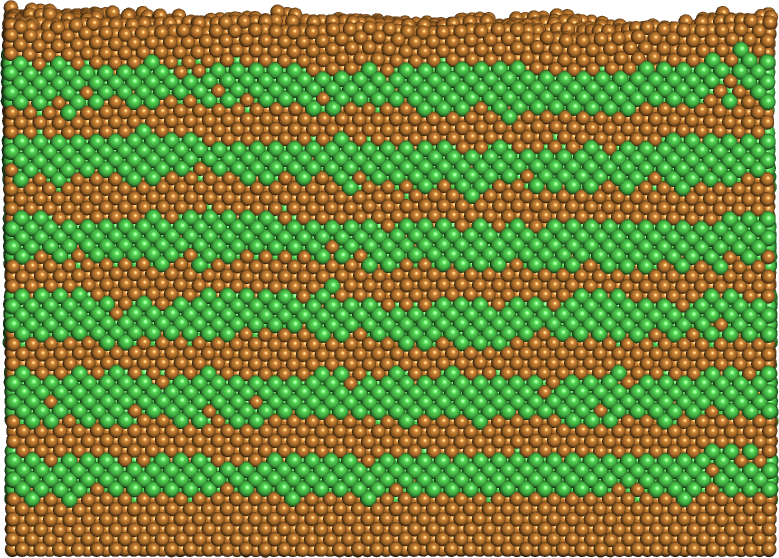
\includegraphics[width=\textwidth]{CuNi_23abit_57_profile}
    \subcaption{Profil von \ce{Cu-Ni}-Multilagen mit Parsivald}
  \end{subfigure}

  \caption{Vergleich von Multilagen-Profilen mit LAMMPS und Parsivald}
  \label{fig:multilayerresults}
  \todoline{Farbcode: Was ist was?}
\end{figure}

\subsection{Vergleich der Parallelisierbarkeit}

Mit beiden Programmen konnte eine Laufzeit von \SI{3.5}{d} für 14 Lagen auf Substraten mit einer Fläche von \SI{106x106}{\angstrom} erzielt werden, wobei der Unterschied in der Zahl der parallelen Prozesse lag.
Während LAMMPS einen kompletten Knoten mit 48 Prozessen ausgelastet hat, liefen die Parsivald-Simulationen mit $p = 4.18$ Prozessen, von denen der Hauptprozess zu weniger als \SI{2}{\percent} ausgelastet war.
Damit erreicht Parsivald für das untersuchte System eine Leistungssteigerung gegenüber reinen LAMMPS-Simulationen um einen Faktor von \num{14}, der für $w_\text{sim} < w_\text{eff}$ sogar quadratisch mit der Breite $w_\text{sim}$ des quadratischen Simulationsraumes zunimmt.

\subsection{Fazit}

Parsivald ermöglicht die effiziente Simulation komplizierter Abscheidungsprozesse wie Multi\-lagen-Abscheidungen mit der gleichen Aussagekraft wie reine MD-Simulationen, benötigt dafür aber weniger als \SI{10}{\percent} der Rechenkapazitäten.
Die Ergebnisse für das epitaktische Wachstum von Kupfer-Nickel-Multilagen mit einer Dicke von je \SI{1}{\nano\meter} stimmen dabei für beide Methoden in Schichtqualität und Rauheit gut überein.

